\section{State Of The Art Analysis}\label{sec:state-of-the-art-analysis}
This section will discuss the state of the art of technologies already used in amusement parks around the world.
It will also focus on those used, or that have been used in the past, in the Mirabilandia park in Italy.
The main purpose is to understand what would be the best ``smart'' and innovative technological options to use in Mirabilandia nowadays considering the Micro City context.
As seen in the documents "Micro City - Domain Analysis" and "Micro City - Case Study Analysis", an Amusement Park as a Micro City has the following necessities:
\begin{itemize}
    \item Queue management: the park may want to offer its visitors the possibility of reducing the waiting time to access an attraction, event or a food service
    \item Personalization of the experience: recommendation systems may be used by the park to suggest attractions, restaurants, events, etc. based on the visitors' interests
    \item Proximity/localization suggestions: visitors may receive on their wearable device some notifications concerning marketing, offers or the queue with fewer wait-time based on their position within the park
\end{itemize}

The following sections are intended to provide an overview of companies' solutions and technologies already used in amusement parks around the world,
as well as Mirabilandia's current offers in terms of smart solutions.

Companies like Accesso and Disney have implemented a system for virtual queueing and recommendation and also something for proximity marketing.

\subsection{Accesso Technology Group}
The main solution adopted by amusement parks to avoid long lines is the \textbf{virtual queueing} system.

Also why: Virtual queuing helps remove the number one frustration of guests (waiting in lines), increasing guest
satisfaction and revenue.
Virtual queuing can add new revenue streams to your organization, and it can also unlock
secondary spending as guests visit F\&B locations or retail locations.
(https://www.accesso.com/learn/virtual-queuing-less-waiting-more-fun)

Also other uses of the virtual queueing (Boston Airport (Accesso), social distancing etc.)

\subsubsection{Lo-Queue Virtual Queueing Products}
Accesso Technology Group\footnote{\url{https://www.accesso.com/}} (formerly Lo-Q) is an English company that provides
devices and mobile apps for virtual queueing to several clients, including theme parks like the ``Six Flags'' corporation in the US
and ``LEGOLAND Windsor Resort'' in the UK\@.
Their technology is patented %TODO

Their products for virtual queueing are \textit{Qsmart} and \textit{Prism}\footnote{\url{https://www.accesso.com/solutions/virtual-queuing/prism}}
and they also used to sell the devices \textit{Qbot} and \textit{Qband} no longer available to this days~\cite{accesso-wikipedia}.
With Qsmart people can access the virtual queueing services directly from their smartphones whereas Prism is a ``smartwatch-like''
wearable.

\subsubsection*{Prism}
The latter is a standalone device, with no need for kiosks or charging stations to support its use.
Moreover, it is waterproof, hypoallergenic, durable and brandable~\cite{prism-desc}.
As can be observed in Figure~\ref{fig:prism}, Prism provides the following functionalities:
\begin{itemize}
    \item Virtual queueing: \textit{visitors} can manage their reservation in line and monitor the line status
    \item Payments: \textit{visitors} can make payments via secure NFC technology
    \item Messaging: \textit{visitors} can receive push notifications for proximity-based marketing (i.e.\ trigger nearby events based on people location, Figure~\ref{fig:prism-icecream}), operational updates, or the status of pending virtual queue positions
    \item Photography: Prism allows automated tagging of ride and park photographs
    \item Access: \textit{visitors} can easily access park turnstiles, guest lockers, resort hotel rooms, etc.
    \item Intelligence: Prism collects real-time information about the users' behaviour during the visit for marketing and park operations purposes
\end{itemize}

\begin{figure}[H]
    \centering
    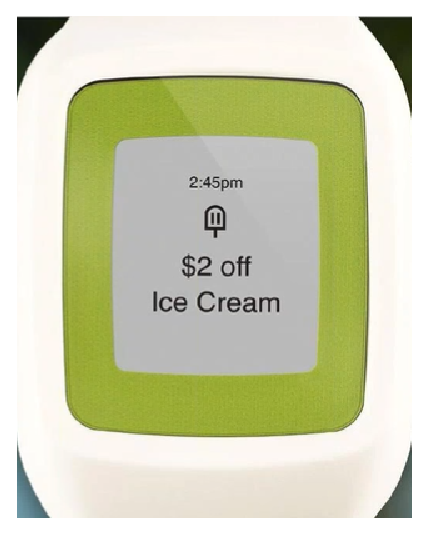
\includegraphics[width=0.3\textwidth]{img/prism-icecream}
    \caption{Example of a push notification based on the visitor proximity to an ice cream shop}
    \label{fig:prism-icecream}
\end{figure}

In addition to their patented virtual queueing technologies, Prism works on a \textbf{proprietary network} and uses three ways to communicate:
\begin{itemize}
    \item \textbf{Bluetooth Low Energy (BLE Beacon):} allows sending real-time messages to \textit{visitors} based on their location, triggers interactions and gain valuable insights about visitors' flow throughout the park
    \item \textbf{Near Field Communication (NFC):} used for access, payments, rentals, etc.
    \item \textbf{Long Range Sub-GHz Two-Way Radio:} allows \textit{visitors} to reserve and modify queueing reservations without having to use their smartphone from where they are
\end{itemize}

The wearable is made with waterproof materials and carries a vibrator motor for haptic feedback to interact with the user and send alerts.
Moreover, its battery supports over 200 days of usage.
Technical specifications~\cite{prism-manual} are listed in Tables~\ref{tab:ci-tec-spec},~\ref{tab:pr-tec-spec},~\ref{tab:c-tec-spec}.

\begin{table}[H]
    \centering
\begin{subtable}[t]{0.85\textwidth}
    \centering
    \begin{tabular}{|l|l|}
        \hline
        LCD & LCD Display, 3 bit colour, Resolution 176 x 176 \\ \hline
        Vibrator motor & 1,000 rpm \\
        \hline
    \end{tabular}
    \caption{Controls and Indicators}
    \label{tab:ci-tec-spec}
\end{subtable}
\begin{subtable}[t]{0.85\textwidth}
    \centering
    \begin{tabular}{|l|l|}
        \hline
        Battery & CR3032 Lithium Ion coin cell \\ \hline
        Average life & 200 days or 2,000 hours \\
        \hline
    \end{tabular}
    \caption{Power Requirements}
    \label{tab:pr-tec-spec}
\end{subtable}
\begin{subtable}[t]{0.85\textwidth}
    \centering
    \begin{tabular}{|l|l|}
        \hline
        Long Range & 868MHz \& 915MHz (SubGHz) transceiver \\ \hline
        Medium Range & 2.4GHz BLE transceiver \\ \hline
        Short Range & Secure 14443 RFID/NFC device \\
        \hline
    \end{tabular}
    \caption{Communications}
    \label{tab:c-tec-spec}
\end{subtable}
    \caption{Prism technical specifications}
    \label{tab:prism-tech-spec}
\end{table}

\subsubsection*{QSmart}
On the other hand, QSmart is a ready-to-use platform and utilizes the visitor's smartphone hardware, is cloud based
and operates via Wi-Fi.

In addition to the features already listed for Prism, Qsmart gives the possibility to easily make rides and
show ticket purchases -- with its mobile payments system which is
PCI\footnote{\url{https://en.wikipedia.org/wiki/Payment_Card_Industry_Data_Security_Standard}} compliant --,
allows choosing among a different set of ride packages with different perks depending on the price, validating the
ride by a QR code and it can be integrated with other Accesso's products like, for instance, an online ticketing system.


\begin{figure}[H]
    \centering
    \begin{subfigure}[b]{0.85\textwidth}
        \centering
        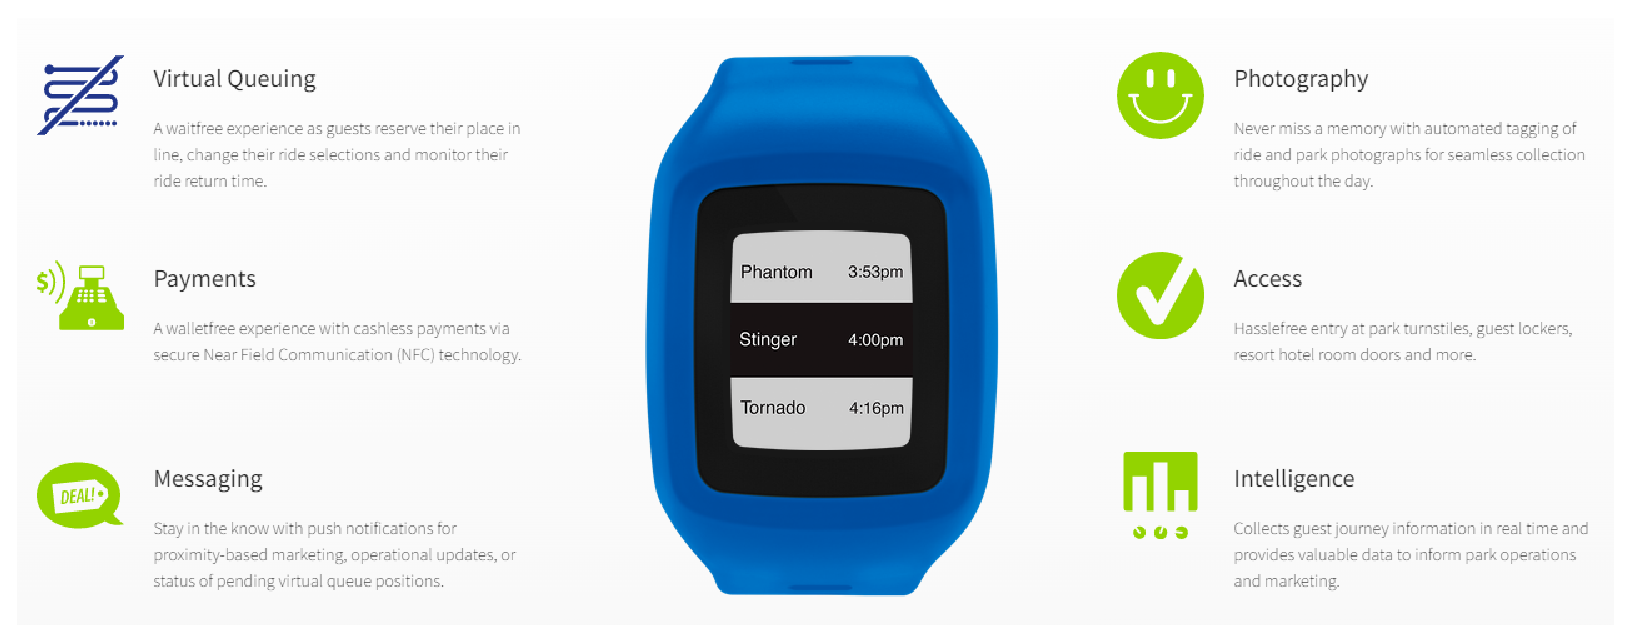
\includegraphics[width=\textwidth]{img/prism}
        \caption{Prism main functionalities}
        \label{fig:prism}
    \end{subfigure}
    \hfill
    \begin{subfigure}[b]{0.85\textwidth}
        \centering
        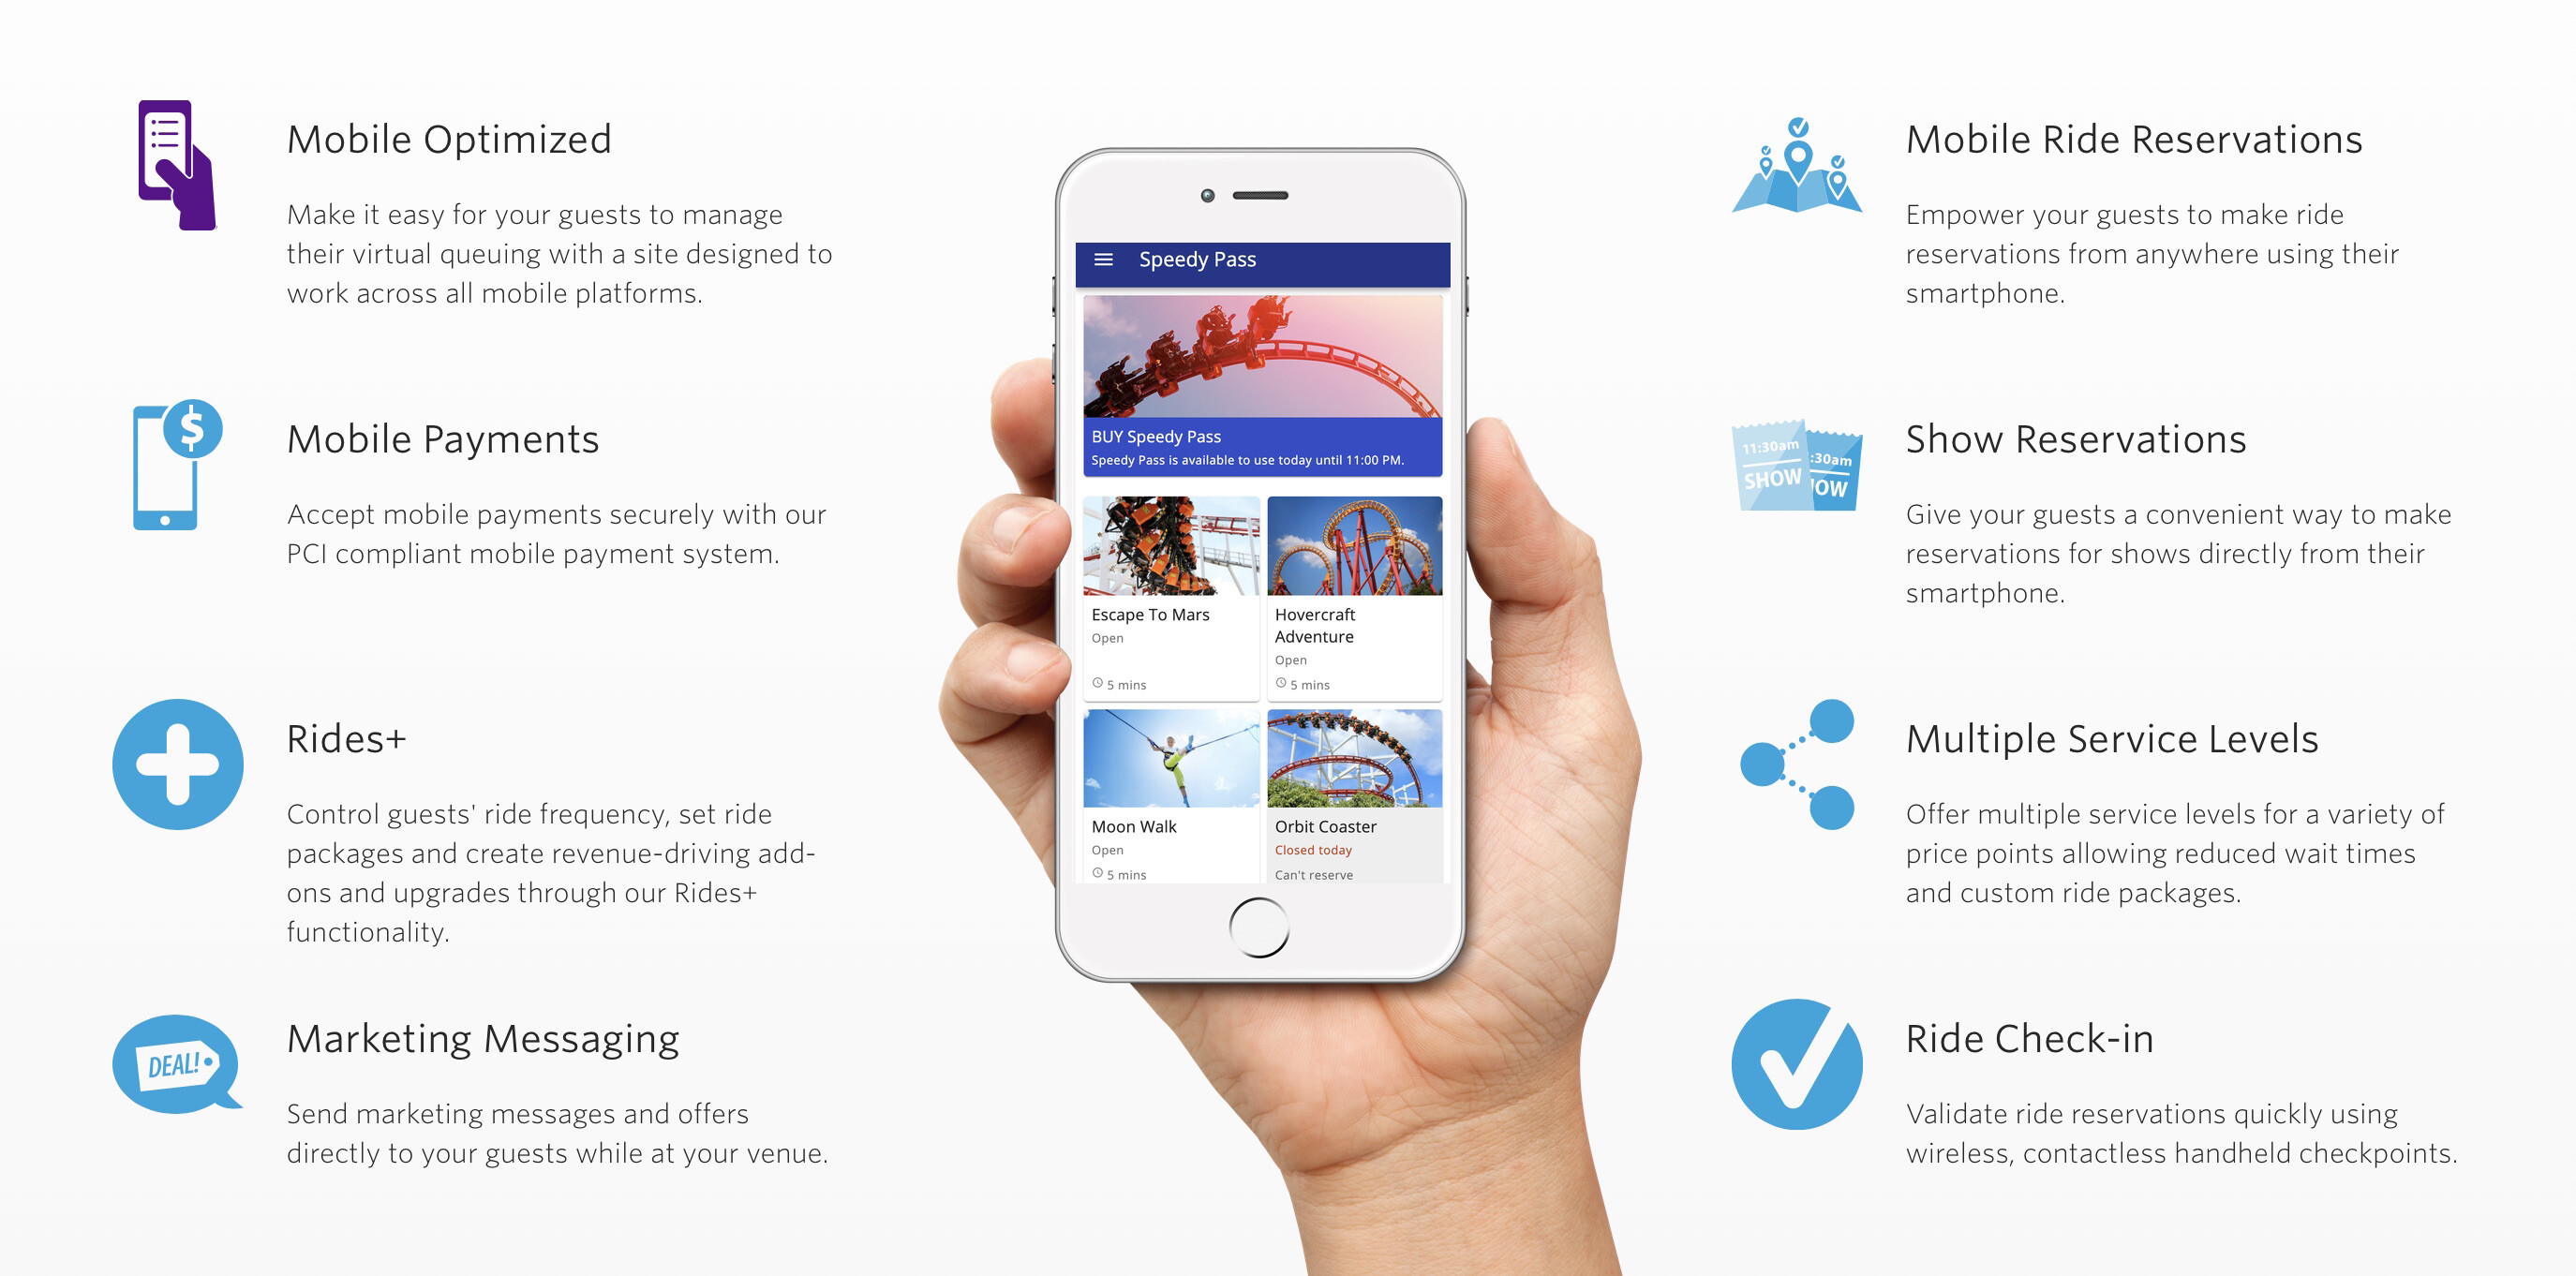
\includegraphics[width=\textwidth]{img/qsmart}
        \caption{Qsmart main functionalities}
        \label{fig:qsmart}
    \end{subfigure}
    \caption{Accesso's products for virtual queueing\protect\footnotemark}
    \label{fig:prismart}
\end{figure}
\footnotetext{\url{https://www.accesso.com/solutions/virtual-queuing}}

Both Prism and QSmart interact with the Virtual Queue Management System, where customers can consult
analytics and performance data as well as centralised data on park attendace.
It is also possible to check ride usage, \textit{visitors} activity, ride downtime and transactional data per user and how log they waited for each ride.
Finally it is possible to control in real-time the virtual queueing solution.
However, there isn't much information about this product on the company website.

They provided their Q-Bot device also to Mirabilandia in 2009 but is no longer used to these days.

\subsubsection{Guest experience management platform}\label{subsec:guest-experience-management-platform}
\subsubsection{Legoland Windsor - Reserve and Ride}\label{subsec:legoland-windsor---reserve-and-ride}

\subsection{Walt Disney Company}\label{subsec:walt-disney-company}

\subsection{Mirabilandia App}\label{subsec:mirabilandia-app}
What Mirabilandia offers nowadays
- fornisce già percorsi specifici per chi è interessato a giochi adrenalinici, per bambini ecc.

